\section{Experimentación}
	Todos los experimentos se repitieron 20 veces. Para reproducirlos se debe ejecutar exp/exp.sh -n 20  

	\subsection{Experimento 1}
		En el primer experimento se genera una serie de imágenes de diferentes tamaños, tomando una imagen grande y disminuyendo progresivamente sus dimensiones.
		Luego, se ejecuta el filtro \emph{blur} con cada una de las imágenes generadas y se compara el tiempo de ejecución de las implementaciones en C y lenguaje ensamblador.
		Esto se repite para el filtro \emph{diff}, con la diferencia de que para cada tamaño de imagen se genera 
		un par de imágenes con ciertas diferencias entre ellas, para poder verificar el buen funcionamiento del mismo.

		\subsubsection*{Hipótesis} 
			Se espera observar que la implementación en lenguaje ensamblador de ambos filtros sea más eficiente, independientemente del tamaño de la imagen. Esto se debe a que hacen uso del modelo \acr{SIMD}, con todas las ventajas ya mencionadas que esto tiene sobre el rendimiento del código, a diferencia de las implementaciones de los algoritmos en C, que procesan cada píxel de manera independiente. Esto último puede inferirse no solo de la estructura propia del código, cuyos ciclos iteran sobre un único píxel a la vez, sino también de la ausencia de instrucciones \acr{SEE} para procesamiento de valores empaquetados que se observa al desensamblar los objetos obtenidos a partir de este código.

		\subsubsection*{Valores utilizados como parámetros} 		
			En este experimento el ancho de las imágenes utilizadas como parámetro se encuentran en un rango entre 24 y 1800 píxeles.Además, para el filtro Blur se utilizó $Radio = 15$ y $Sigma = 5$.

		\subsubsection*{Resultados}
		   	{\centering \begin{tabular}{c}
		      {\small Filtro Diferencia} \\
		      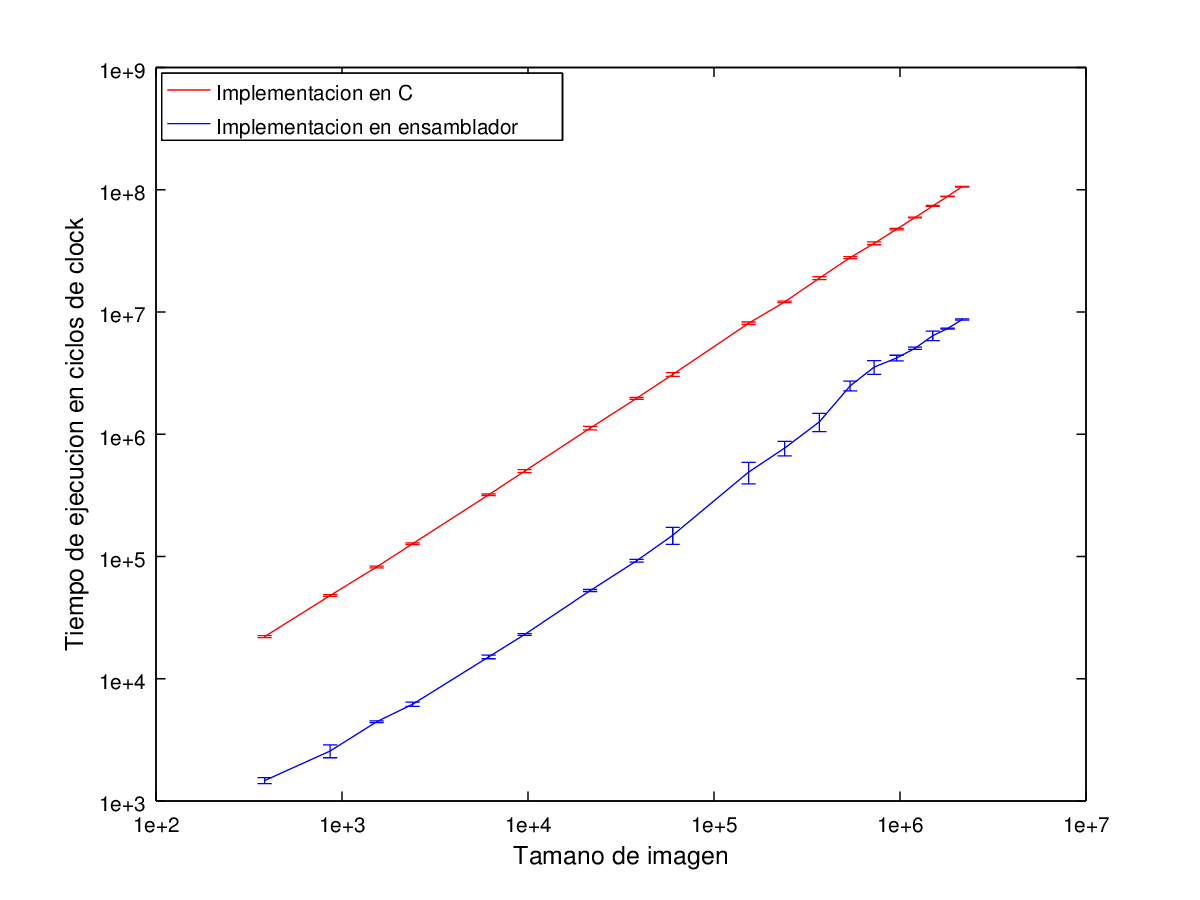
\includegraphics[width=12cm]{../exp/graficos/exp1-diff-c_vs_asm.png} \\
		    \end{tabular}}

		    {\centering \begin{tabular}{c}
		      {\small Filtro Diferencia - Tiempo de ejecución normalizado por píxel} \\
		      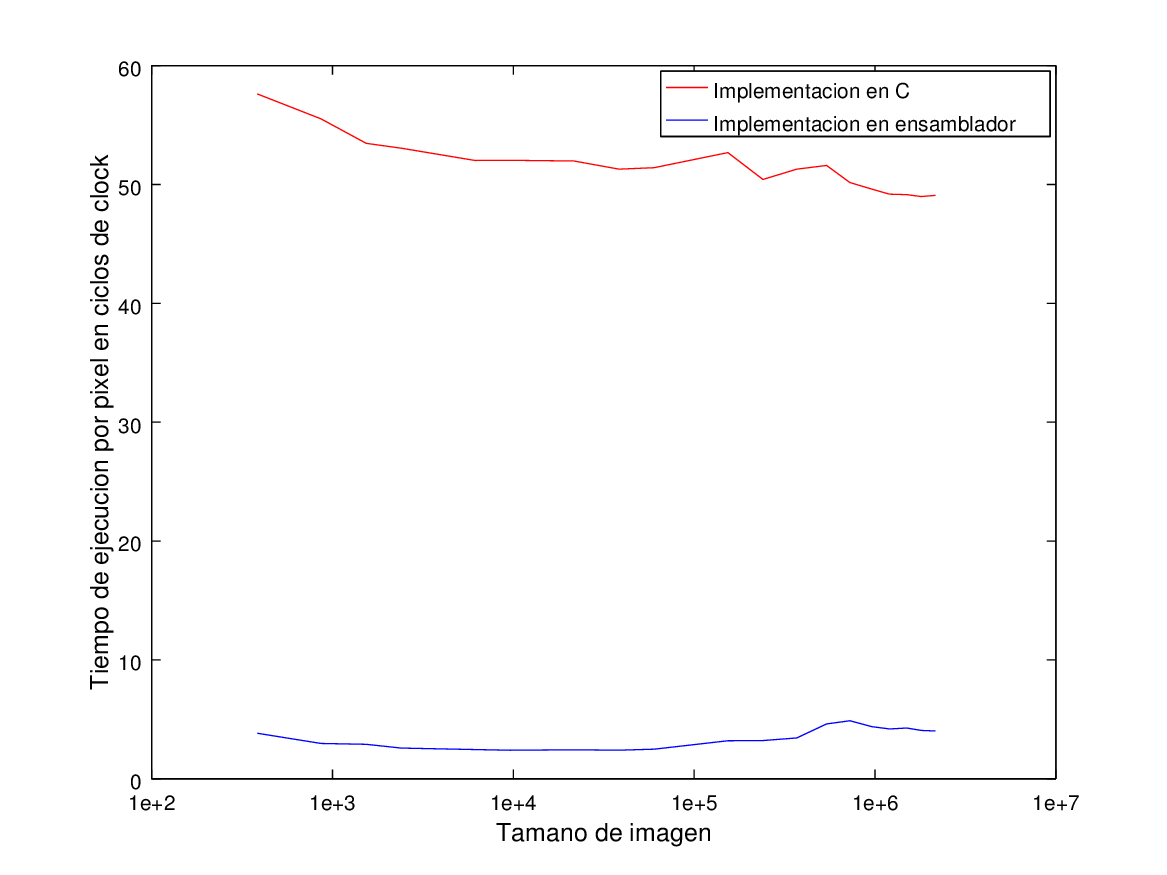
\includegraphics[width=12cm]{../exp/graficos/exp1-diff-tiempo_por_pixel.png} \\
		    \end{tabular}}

			{\centering \begin{tabular}{c}
		      {\small Filtro Blur} \\
		      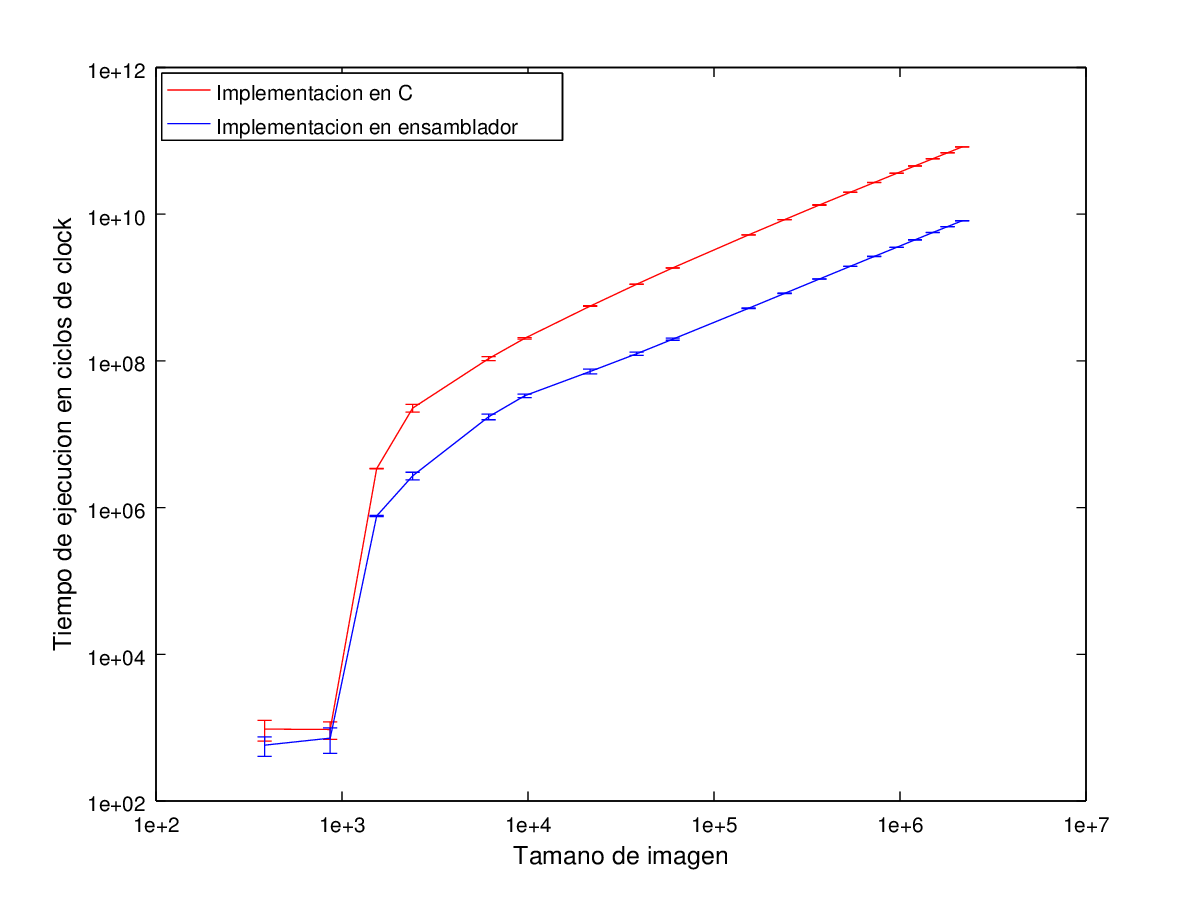
\includegraphics[width=12cm]{../exp/graficos/exp1-blur-c_vs_asm.png} \\
		    \end{tabular}}

		   	{\centering \begin{tabular}{c}
		      {\small Filtro Blur - Tiempo de ejecución normalizado por píxel} \\
		      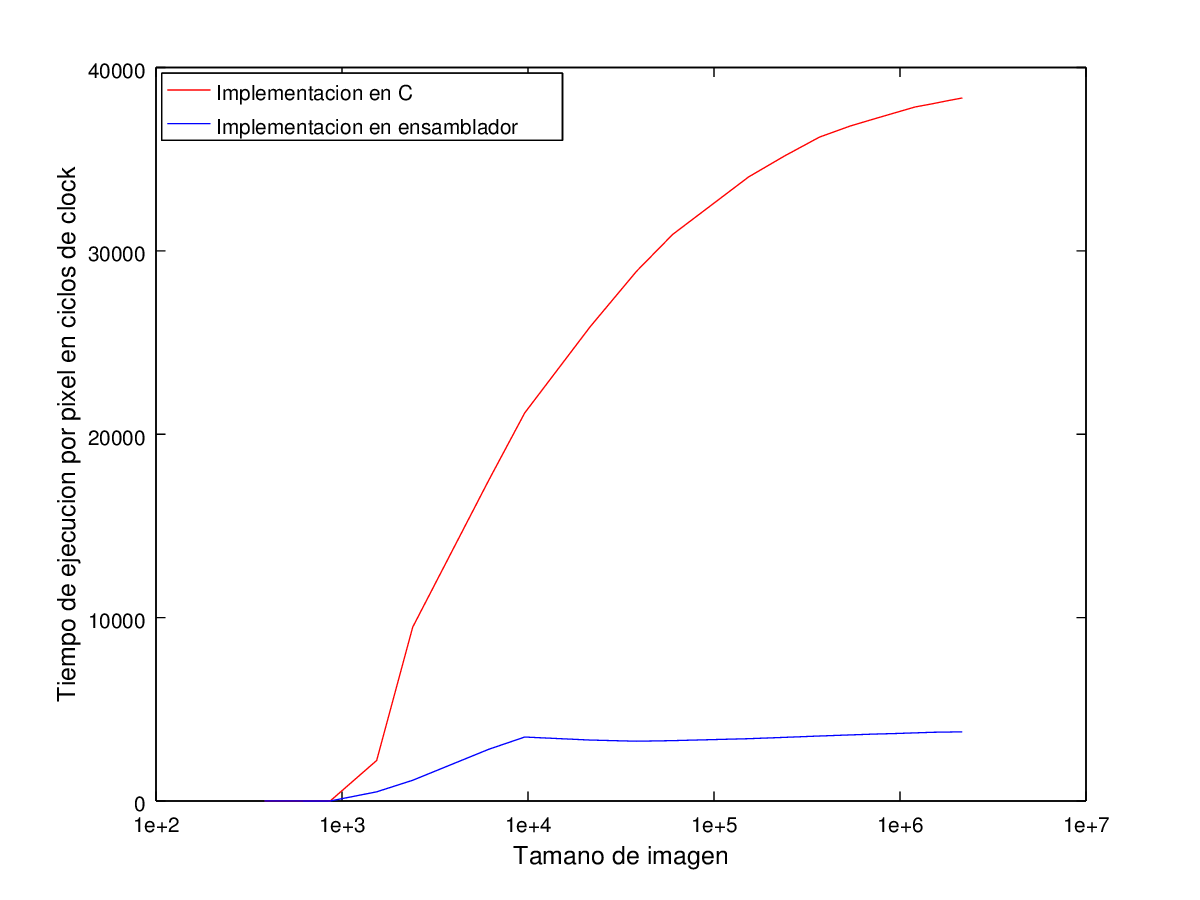
\includegraphics[width=12cm]{../exp/graficos/exp1-blur-tiempo_por_pixel.png} \\
		    \end{tabular}}

		\subsubsection*{Conclusiones y observaciones} 
			Como se observa en los resultados, se pudo confirmar la hipótesis planteada: la implementación en lenguaje ensamblador resultó más rápida que la implementación en C para todos los tamaños de imagen.
			En \emph{blur}, cuando llamamos a la función con un valor de $r$ mayor a la mitad de la altura o a la mitad del ancho de la imagen, no se producen cambios. Dado que en el experimento el valor de $r$ se mantiene constante, las dos imágenes más pequeñas no se ven afectadas por el filtro, lo cual se ve reflejado en los resultados, ya que para estas dos imágenes el tiempo de ejecución es notablemente menor.

	\subsection{Experimento 2}
		El objetivo de este experimento es observar como se ve afectada la eficiencia del algoritmo \emph{blur}, en ambas implementaciones, para diferentes valores del parámetro $r$ manteniendo constante la imagen de entrada.

		\subsubsection*{Hipótesis} 
			Se conjetura que, a medida que el valor del radio $r$ se incrementa, el tiempo de ejecución en las dos implementaciones aumentará, y que lo hará de manera cuadrática con respecto al incremento en $r$. Esto se debe a que la complejidad temporal de cada ejecución del ciclo principal del algoritmo depende del tamaño de la matriz de convolución, que es $(2 \times \mathtt{radio} + 1) \times (2 \times \mathtt{radio} + 1) \times 4$, es decir, es cuadrático en el valor de $r$.

		\subsubsection*{Valores utilizados como parámetros} 
		La dimensión de la imagen utilizada es 400 filas y 600 columnas. El valor del sigma es 5 y los radios toman valores entre 1 y 40.

		\subsubsection*{Resultados}

			{\centering \begin{tabular}{c}
	      		{\small Filtro Blur - Tiempo de ejecución según radio} \\
	      		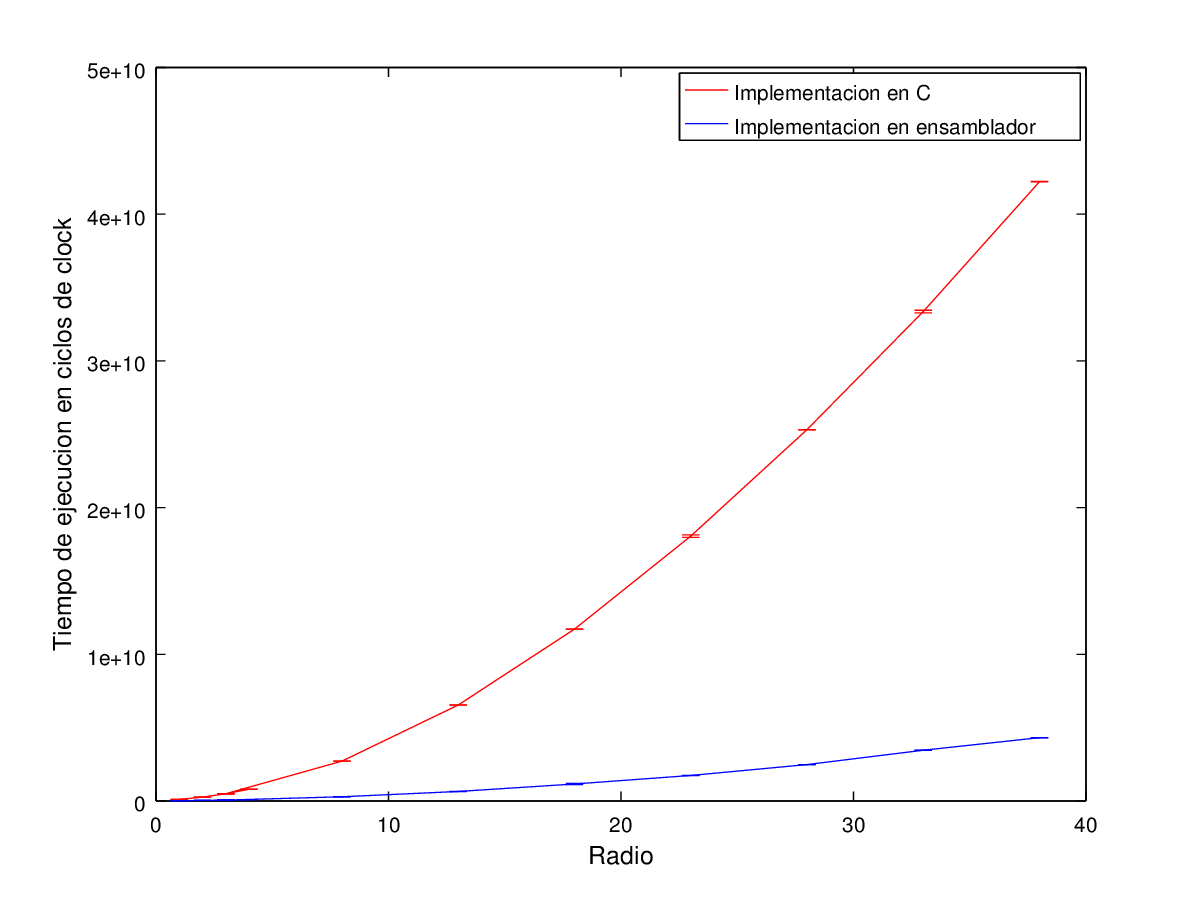
\includegraphics[width=12cm]{../exp/graficos/exp2-tiempo_segun_radio.png} \\
	    	\end{tabular}}

		\subsubsection{Conclusiones y observaciones}
			Se puede observar en los gráficos que a medida que los $r$ aumenta, también lo hace el tiempo de ejecución. En este sentido, se pudo confirmar la hipótesis. Sin embargo, si se dividen los valores del tiempo de ejecución por su correspondiente $r^2$, se comprueba que la relación no es lineal; es decir, el tiempo de ejecución no varía cuadráticamente con el valor de $r$.


	\subsection{Experimento 3}
		Este experimento es similar al anterior, también se realiza sobre las dos implementaciones del filtro \emph{blur} y se considera siempre la misma imagen. En este caso el radio se mantiene constante pero el valor del sigma se modifica. También se va a utilizar el resultado normalizado, para poder estudiar el tiempo de procesamiento por píxel. 

			\subsubsection*{Hipótesis} 
				Debido a que el valor del sigma es utilizado solamente para realizar un cálculo por cada posición de la matriz de convolución, suponemos que modificar este valor no alterará el tiempo de ejecución.

			\subsubsection*{Valores utilizados como parámetros} 
			La dimensión de la imagen utilizada es 400 filas y 600 columnas. El valor del radio es 10 y sigma toma valores entre 0.5 y 50.

			\subsubsection*{Resultados}

			{\centering \begin{tabular}{c}
	      		{\small Filtro Blur - Tiempo de ejecución según sigma} \\
	      			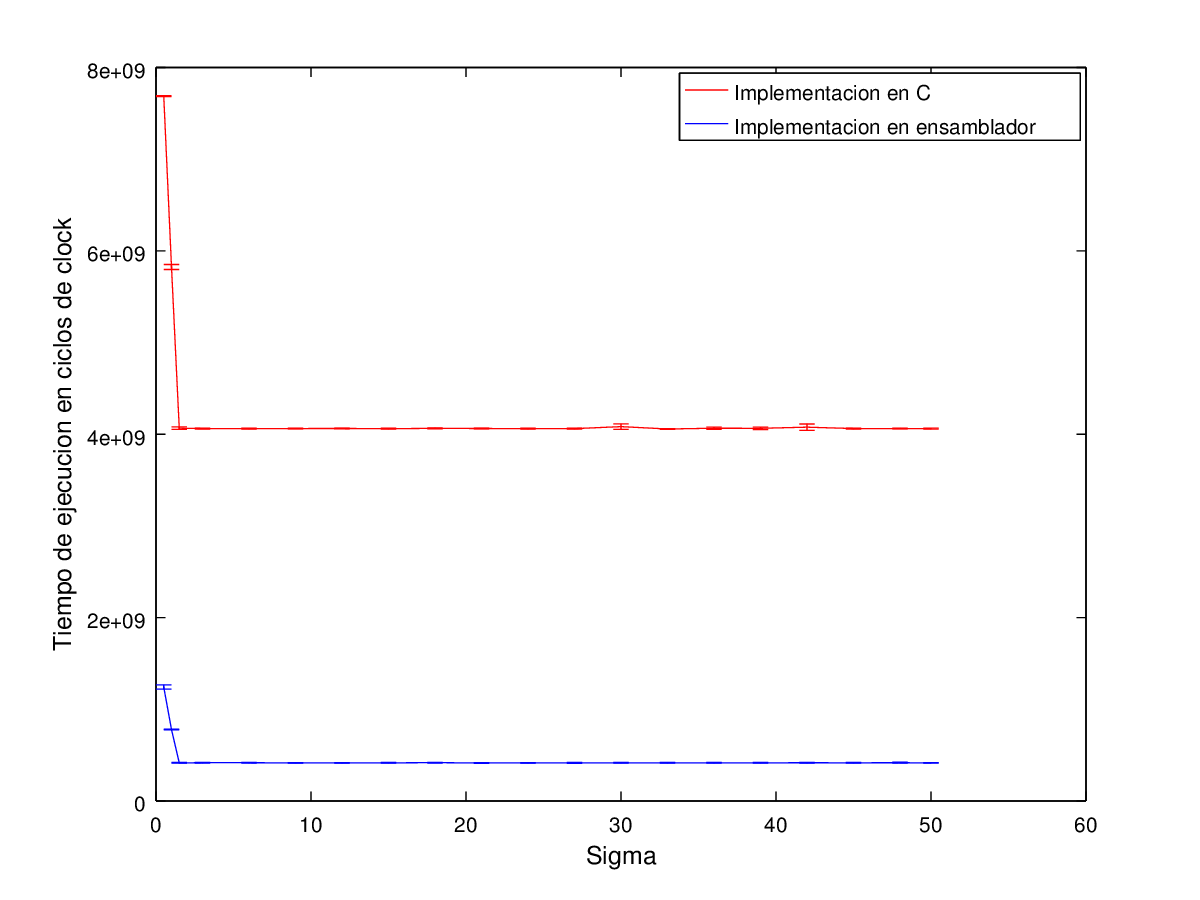
\includegraphics[width=12cm]{../exp/graficos/exp3-tiempo_segun_sigma.png} \\
	    		\end{tabular}}

			\subsubsection*{Conclusiones y observaciones}
				Como dijimos en la hipótesis, la variación del sigma no afecta el tiempo de ejecución del algoritmo, tanto en lenguaje ensamblador como en C. Para valores de sigma menores que 1 podemos observar que el tiempo de ejecución es mayor.

				Esto se debe a que los valores serán muy grandes y el tiempo de ejecución de una cuenta aritmética deja e ser despreciable. 

	\subsection{Experimento 4}
		Otras de las pruebas consiste en comparar los tiempos de ejecución de diferentes implementaciones de los filtros en lenguaje ensamblador. Nos interesa medir el peso que tienen en el tiempo de ejecución los llamados a funciones auxiliares. Para esto, queremos comparar el rendimiento de una implementación que utiliza llamados a estas funciones, con el de otra que tiene todas las instrucciones necesarias en el mismo bloque de código (sin utilizar esas funciones auxiliares). 
		
		Este experimento se realiza una determinada cantidad de veces con distintos tamaños de imagen.

			\subsubsection*{Hipótesis} 
				Creemos que la versión del código implementada en lenguaje ensamblador que no realiza llamados a funciones va a tener un mejor rendimiento, ya que se evita el overhead que producen estos llamados.
		
			\subsubsection*{Valores utilizados como parámetros} 
				En este experimento el ancho de las imágenes utilizadas como parámetro se encuentran en un rango entre 24 y 1800 píxeles.Además, para el filtro Blur se utilizó $Radio = 15$ y $Sigma = 5$.


			\subsubsection*{Resultados}
				{\centering \begin{tabular}{c}
		      		{\small Filtro Diferencia} \\
		      		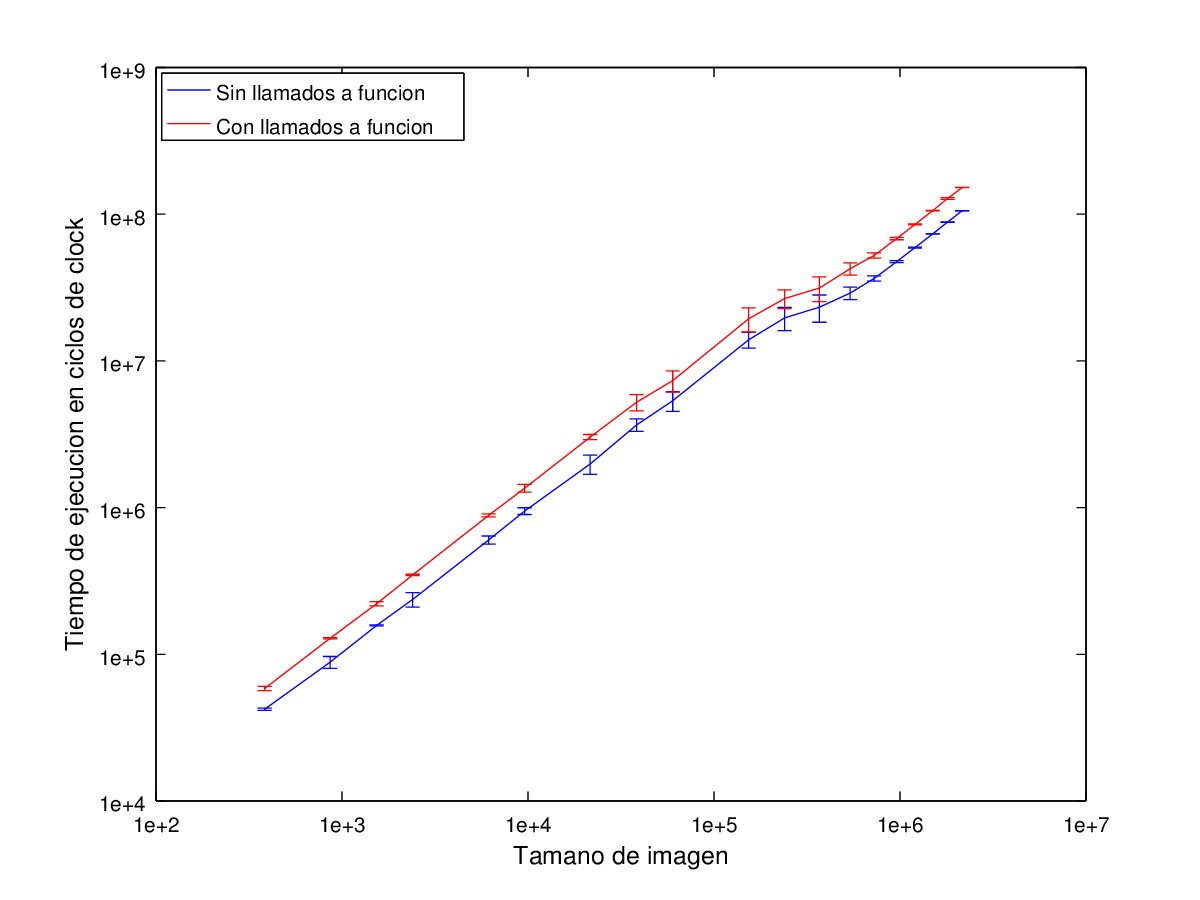
\includegraphics[width=12cm]{../exp/graficos/exp4-diff-c_vs_c2.png} \\
		    	\end{tabular}}

				{\centering \begin{tabular}{c}
		      		{\small Filtro Blur} \\
		      		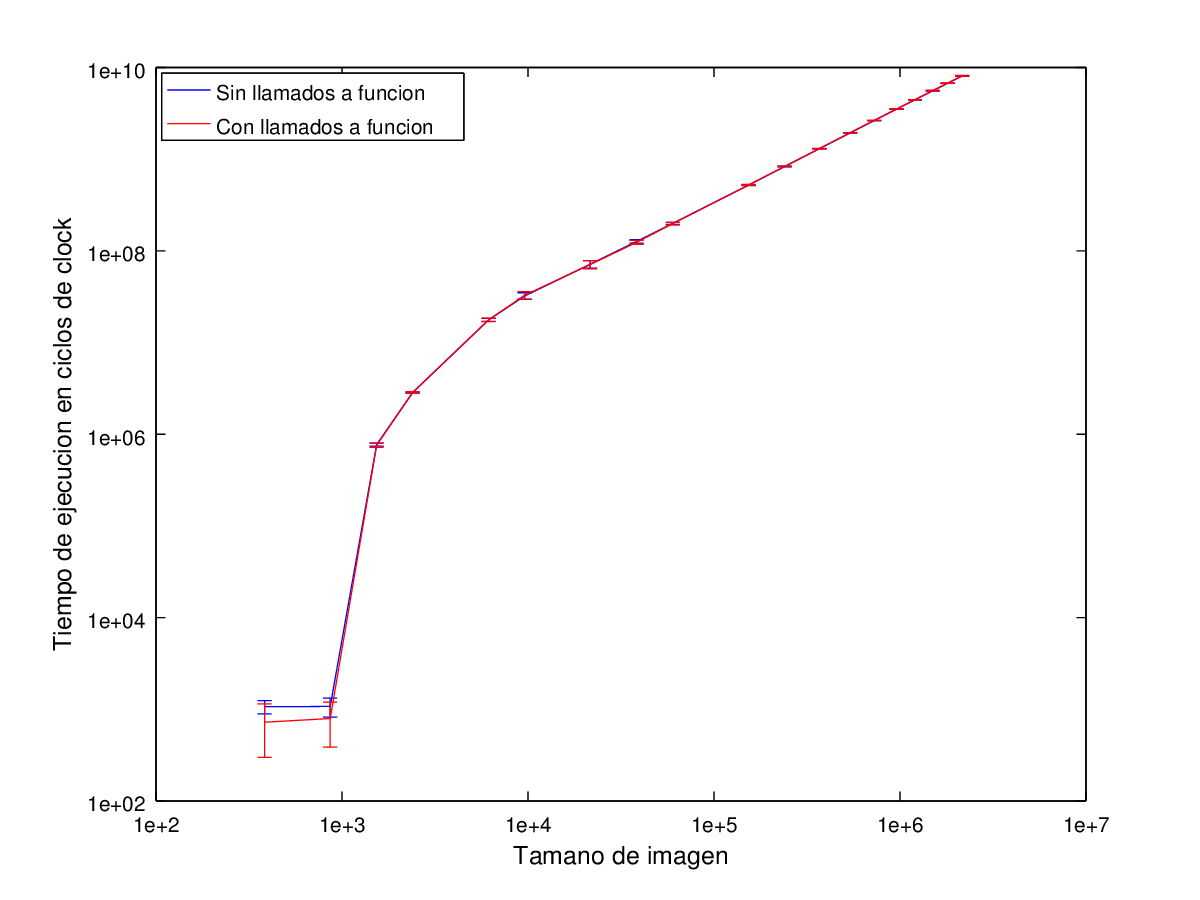
\includegraphics[width=12cm]{../exp/graficos/exp4-blur-asm_vs_asm2.png} \\
		    	\end{tabular}}

			\subsubsection*{Conclusiones y observaciones}		

				Como muestran los gráficos de la implementación en C, los algoritmos que hacen llamados a otras funciones tienen un mayor tiempo de ejecución que las que no los hacen. Esto se debe a que cada vez que se hace un llamado a función, en necesario modificar la pila, manteniéndola alineada y guardando los registros que se deben preservar según la convención C y fueron utilizados a lo largo de la función.

				En lenguaje ensamblador, cuando implementamos el algoritmo sin el llamado a la función auxiliar, sigue siendo necesario acceder a la pila ya que hay que reutilizar registros que se tienen que mantener para la convención C. Por esto, seguimos haciendo accesos a memoria. Una vez que la accedemos es muy posible que en la cache se encuentren los siguientes accesos a realizar. Entonces la diferencia entre accederla unas pocas veces o mas es muy similar, ya que el acceso a memoria cache no es muy caro.

				Escribir un código en donde no realizamos llamadas a funciones auxiliares es mas difícil de mantener y además queda mas legible.
